\scalebox{1}{
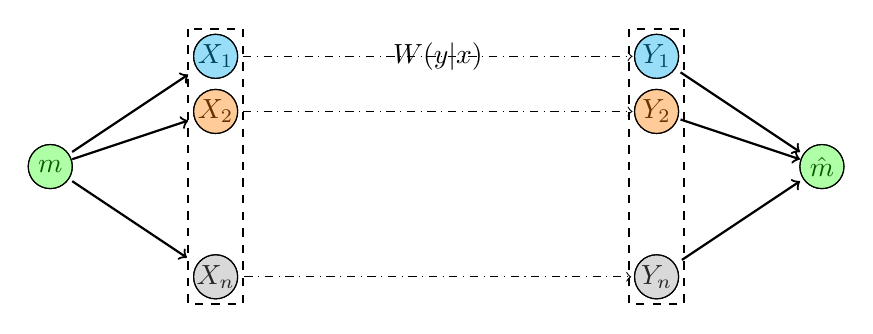
\begin{tikzpicture}[scale=.7][thick]


\draw [thick,dashed] (-4.5,4) rectangle (-3.5,-1);
\draw (-4,3.5) circle (.4cm);
\node[] at (-4,3.5) (X_1) {$X_1$};

\draw (-4,2.5) circle (.4cm);
\node[] at (-4,2.5) (X_2) {$X_2$};
\draw (-4,-.5) circle (.4cm);
\node[] at (-4,-.5) (X_n) {$X_n$};




\draw (-7,1.5) circle (.4cm);

\node[] at (-7,1.5) (m) {$m$};
\draw[thick,->] (m) -- (X_1);
\draw[thick,->] (m) -- (X_2);
\draw[thick,->] (m) -- (X_n);


%%%%%%%%%%%%%%%%%%%%%%%%%%%%%%%%%%%%%%
\draw [thick,dashed] (4.5,4) rectangle (3.5,-1);
\draw (4,3.5) circle (.4cm);
\node[] at (4,3.5) (Y_1) {$Y_1$};\draw (4,2.5) circle (.4cm);
\node[] at (4,2.5) (Y_2) {$Y_2$};
\draw (4,-.5) circle (.4cm);
\node[] at (4,-.5) (Y_n) {$Y_n$};

\draw (7,1.5) circle (.4cm);

\node[] at (7,1.5) (m) {$\hat{m}$};
\draw[thick,->] (Y_1) -- (m);
\draw[thick,->] (Y_2) -- (m);
\draw[thick,->] (Y_n) -- (m);

\draw [dashed,dash dot,->] (X_1) -- node {$W(y|x)$} (Y_1);
\draw [dashed,dash dot,->] (X_2) -- (Y_2);
\draw [dashed,dash dot,->] (X_n) -- (Y_n);


\draw [fill=green!90!yellow, fill opacity=0.35] (-7,1.5) circle (.4cm);
\draw [fill=green!90!yellow, fill opacity=0.35] (7,1.5) circle (.4cm);

\draw [fill=cyan, fill opacity=0.4] (-4,3.5) circle (.4cm);
\draw [fill=cyan, fill opacity=0.4] (4,3.5) circle (.4cm);

\draw [fill=orange, fill opacity=0.4] (-4,2.5) circle (.4cm);
\draw [fill=orange, fill opacity=0.4] (4,2.5) circle (.4cm);

\draw [fill=gray, fill opacity=0.3] (-4,-.5) circle (.4cm);
\draw [fill=gray, fill opacity=0.3] (4,-.5) circle (.4cm);



\end{tikzpicture}
}